\documentclass[journal,twocolumn]{IEEEtran}

\usepackage[utf8]{inputenc}
\usepackage{amsmath,amssymb,amsfonts}
\usepackage{graphicx}
\usepackage{booktabs}
\usepackage{cite}
\usepackage{microtype}
\usepackage{tabularx}
\usepackage{multirow}
\usepackage{xcolor}
\usepackage[colorlinks=true,linkcolor=blue,citecolor=blue,urlcolor=blue]{hyperref}
\usepackage{cleveref}

\DeclareMathOperator*{\argmax}{arg\,max}
\DeclareMathOperator*{\argmin}{arg\,min}
\newcommand{\APOE}{\textit{APOE}}

\begin{document}

\title{Multimodal Deep Learning and Graph Representation of 3D Brain MRI with Genomic Conditioning for Alzheimer's Disease Progression: Benchmarks, Leakage Audits, and Longitudinal Forecasting}

\author{Dhriti~Gandhi,
        Ura~Modi,
        Devashree~Parikh,
        Yash~Shah,
        and~Mehul~S.~Raval,~\IEEEmembership{Senior Member,~IEEE}%
\thanks{The authors are with the School of Engineering and Applied Sciences, Ahmedabad University, Ahmedabad, Gujarat 380009, India (e-mail: mehul.raval@ahduni.edu.in).}%
\thanks{Data used in preparation of this article were obtained from the Alzheimer's Disease Neuroimaging Initiative (ADNI) database (\url{adni.loni.usc.edu}).}}

\markboth{IEEE Transactions on Medical Imaging / arXiv Preprint, November~2026}%
{Gandhi \MakeLowercase{\textit{et al.}}: Multimodal Neuroimaging-Genomic Learning for Alzheimer's Disease Progression}

\maketitle

\begin{abstract}
Tracking Alzheimer's Disease (AD) progression requires mapping high-dimensional 3D structural neuroimaging and genetic risk ($\APOE\ \varepsilon4$) to cognitive severity, longitudinal decline, and clinical diagnostic transitions. However, machine learning in neuroimaging is frequently plagued by optimistic performance reporting driven by subtle subject-level data leakage, unconstrained deep voxel embeddings, and poorly characterized temporal modeling. In this work, we present a leak-free, multimodal deep learning framework evaluated on a curated cohort of 394 longitudinally segmented 3D T1-weighted MPRAGE MRI scans from 204 unique ADNI participants. We systematically benchmark regularized tabular morphometry, 3D Vision Transformers (ConvViT3D), and Graph Attention Networks with learned edge sparsity (GATv3) across three core clinical tasks: (1) Static Cognitive Severity Regression, where our models explain up to $68.0\%$ of cognitive variance ($R^2 = 0.680$, $95\%$ bootstrap CI: $[0.571, 0.759]$ on ADAS-Cog13, $R^2 = 0.639$ on CDR-SB, and $R^2 = 0.625$ on MMSE); (2) Temporal Forecasting, where models accurately predict 1-year future cognitive level ($R^2_{\text{level}} = 0.788$) and identify significant $\APOE \times \text{time}$ acceleration interactions ($p = 2.05 \times 10^{-8}$), while highlighting the mathematical limits of predicting 1-year change deltas ($\Delta R^2 \approx 0.03 - 0.08$); and (3) Diagnostic and Rapid Decline Classification, where multi-compartment neural fusion reaches $\text{AUC} = 0.972$ (and ExtraTrees reaches $\text{AUC} = 0.979$) for Cognitively Normal vs.\ AD dementia, and $\text{AUC} = 0.785$ for 1-year rapid clinical decline. Crucially, a 6-protocol leakage audit ($P_0 - P_5$) demonstrates that naive scan-level splitting inflates regression $R^2$ by $+0.094$ on real clinical targets and introduces an artificial $+0.155$ inflation on permuted null targets, exposing patient identity memorization. Our findings provide a rigorous, reproducible benchmark for trustworthy multimodal AI in dementia care.
\end{abstract}

\begin{IEEEkeywords}
Alzheimer's Disease, 3D T1-weighted MRI, Graph Attention Networks, 3D Vision Transformers, Data Leakage Audit, Longitudinal Forecasting, Multimodal Fusion.
\end{IEEEkeywords}

\section{Introduction}
\IEEEPARstart{A}{lzheimer's} Disease (AD) represents the leading cause of dementia worldwide, characterized neurobiologically by amyloid-$\beta$ plaques, neurofibrillary tau tangles, and progressive macroscopic brain atrophy \cite{jack2018nia, scheltens2021alzheimer}. Clinically, patients transition from Cognitively Normal (CN) status through Mild Cognitive Impairment (MCI) to terminal dementia. Developing reliable computer vision and machine learning frameworks capable of staging current cognitive severity, predicting longitudinal trajectories, and detecting clinical transitions is essential for timely patient counseling and clinical trial enrichment \cite{frisoni2010clinical}.

Over recent years, multimodal neuroimaging-genomic learning has gained substantial traction \cite{dolci2025interpretable, chakraborty2020deep}. High-resolution 3D T1-weighted structural Magnetic Resonance Imaging (sMRI) provides non-invasive spatial measurements of neurodegeneration, while the Apolipoprotein E ($\APOE$) $\varepsilon4$ allele represents the preeminent genetic risk factor for late-onset AD \cite{cordeau2020apoe}.

However, despite reports of high predictive accuracy, translated clinical utility remains scarce due to three foundational challenges:
\begin{enumerate}
    \item \textbf{Subject-Level Data Leakage:} When multi-visit longitudinal scans from the same individual are split randomly across training and testing sets, models memorize idiosyncratic patient anatomy rather than disease pathology, producing severely inflated performance estimates \cite{wen2020convolutional, yagis2021effect}.
    \item \textbf{The Representation Gap (Voxel vs.\ Graph Morphometry):} Unconstrained 3D deep neural networks (CNNs, Vision Transformers) struggle on sample sizes typical of medical cohorts ($N \sim 10^2 - 10^3$), whereas biologically grounded cortical parcellations and anatomical Graph Neural Networks (GNNs) provide structured inductive biases.
    \item \textbf{The Level vs.\ Delta Dilemma in Longitudinal Modeling:} Predicting the absolute future disease severity (level) is often conflated with predicting the 1-year rate of change ($\Delta$). While future score levels can be predicted with high precision ($R^2 \approx 0.79$), predicting short-term deltas is constrained by slow biological progression and psychometric noise.
\end{enumerate}

\paragraph{Contributions} To resolve these challenges, we evaluate a strictly leak-free, patient-grouped framework on a curated cohort of 394 longitudinally segmented 3D T1-weighted MRI scans across 204 unique ADNI participants. Our contributions are:
\begin{itemize}
    \item \textbf{Task 1 (Static Severity Regression):} We achieve peak cross-validated $R^2 = 0.680$ ($95\%$ bootstrap CI: $[0.571, 0.759]$) for ADAS-Cog13, $R^2 = 0.639$ ($[0.517, 0.749]$) for CDR-SB, and $R^2 = 0.625$ ($[0.508, 0.709]$) for MMSE using $\APOE$-conditioned Graph Attention Networks (GATv3) and tabular ensembles.
    \item \textbf{Task 2 (Temporal Progression Regression):} We demonstrate that predicting 1-year future cognitive level achieves $R^2_{\text{level}} = 0.788$, while dissecting why 1-year annualized change deltas yield lower explained variance ($\Delta R^2 \approx 0.03 - 0.08$). We formally verify the $\APOE\ \varepsilon4 \times \text{time}$ acceleration interaction ($p = 2.05 \times 10^{-8}$).
    \item \textbf{Task 3 (Diagnostic and Rapid Decline Classification):} We attain $\text{AUC} = 0.972$ (and ExtraTrees $\text{AUC} = 0.979$) for CN vs.\ AD classification, and $\text{AUC} = 0.785$ for forecasting 1-year rapid cognitive deterioration.
    \item \textbf{The 6-Protocol Leakage Audit ($P_0 - P_5$):} We mathematically isolate the mechanics of data leakage, demonstrating that scan-level splitting inflates Gradient Boosting $R^2$ by $+0.094$ on real targets and by $+0.155$ on permuted noise targets.
\end{itemize}

\section{Cohort and Preprocessing Pipeline}
\label{sec:cohort}

\subsection{Study Cohort}
Data were acquired from the Alzheimer's Disease Neuroimaging Initiative (ADNI). We analyzed a core cohort of 394 longitudinally tracked 3D T1-weighted MPRAGE scans from 204 unique participants, with matched clinical evaluations (MMSE, CDR-SB, ADAS-Cog13) and $\APOE$ genotype ($0, 1,$ or $2$ $\varepsilon4$ alleles).

\subsection{Image Preprocessing and Multi-Compartment Extraction}
\begin{enumerate}
    \item \textbf{Deep Skull-Stripping:} Raw 3D T1 NIfTI volumes were brain-extracted using HD-BET \cite{isensee2019automated}, a 3D U-Net ensemble that eliminates skull and dura while rigorously preserving outer cortical surfaces.
    \item \textbf{Anatomical Parcellation (FastSurfer):} Brain volumes were segmented using FastSurfer \cite{henschel2020fastsurfer} to extract the Desikan-Killiany-Tourville (DKT) atlas, yielding 230 regional morphological features (cortical thickness, gray matter volume, surface area, and subcortical volumes). Volumetric features were normalized to total intracranial volume (ICV).
    \item \textbf{Deep Visual Representation (MedicalNet 3D ResNet):} Brain scans were passed through a 3D ResNet-50 pre-trained on diverse medical datasets (MedicalNet \cite{chen2019med3d}) to extract high-dimensional deep visual embeddings.
    \item \textbf{Medial Temporal Lobe (MTL) Crops:} $64 \times 64 \times 64$ voxel regions centered around the bilateral hippocampus and entorhinal cortex were extracted for 3D Vision Transformers.
\end{enumerate}

\section{Methodology}
\label{sec:methodology}

\subsection{Architectural Spectrum}
\paragraph{Tabular Reference Ensembles} Ridge regression with nested generalized cross-validation (GCV), Extremely Randomized Trees (ExtraTrees), and Histogram Gradient Boosting (HistGBM).
\paragraph{3D Vision Transformers (ConvViT3D)} A hybrid network comprising three 3D convolutional downsampling blocks followed by four 3D Multi-Head Self-Attention layers operating on MTL voxel tokens, concatenated with genotype embeddings.
\paragraph{Graph Attention Networks with Learned Concrete Sparsity (GATv3)} The brain is modeled as an attributed graph $\mathcal{G} = (\mathcal{V}, \mathcal{E})$ with 68 cortical DKT nodes. Multi-head graph attention weights are modulated by stochastic binary gates sampled via the Hard Concrete relaxation \cite{louizos2017learning}:
\begin{equation}
    \alpha_{uv}^{(k)} = \frac{\exp\left(\text{LeakyReLU}\left(\mathbf{a}_k^T [\mathbf{W}_k \mathbf{h}_u \,\|\, \mathbf{W}_k \mathbf{h}_v]\right)\right)}{\sum_{w \in \mathcal{N}(u)} \exp\left(\text{LeakyReLU}\left(\mathbf{a}_k^T [\mathbf{W}_k \mathbf{h}_u \,\|\, \mathbf{W}_k \mathbf{h}_w]\right)\right)} \cdot z_{uv}.
\end{equation}
\paragraph{Multi-Compartment Neural Late Fusion} Out-of-fold probability distributions from tabular, graph, and visual models are fused via a regularized neural meta-learner.

\subsection{The 6-Protocol Leakage Audit Framework}
To audit cross-validation hygiene, we formulated six protocols on $N=364$ scans across $N=200$ subjects:
\begin{itemize}
    \item $P_0$ (Honest): Grouped by subject; all scaling and PCA computed strictly inside training folds.
    \item $P_{0b}$: As $P_0$, with in-fold feature selection.
    \item $P_1$ (Scan Split): Standard KFold over scans (longitudinal visits of the same subject split across train/test).
    \item $P_2$ (Transductive PCA): Scaler and PCA fitted on all scans prior to subject splitting.
    \item $P_3$ (Transductive Selection): Feature selection by target correlation performed across all scans prior to splitting.
    \item $P_5$ (Compound April-Style): Scan split $+$ transductive PCA $+$ global feature selection.
\end{itemize}
Each protocol was evaluated over 30 repetitions on real MMSCORE targets and 15 repetitions on permuted null targets (shuffled across subjects). Under valid validation, expected null $R^2$ must be $\le 0$.

\section{Experimental Results}
\label{sec:results}

\begin{figure}[t]
\centering
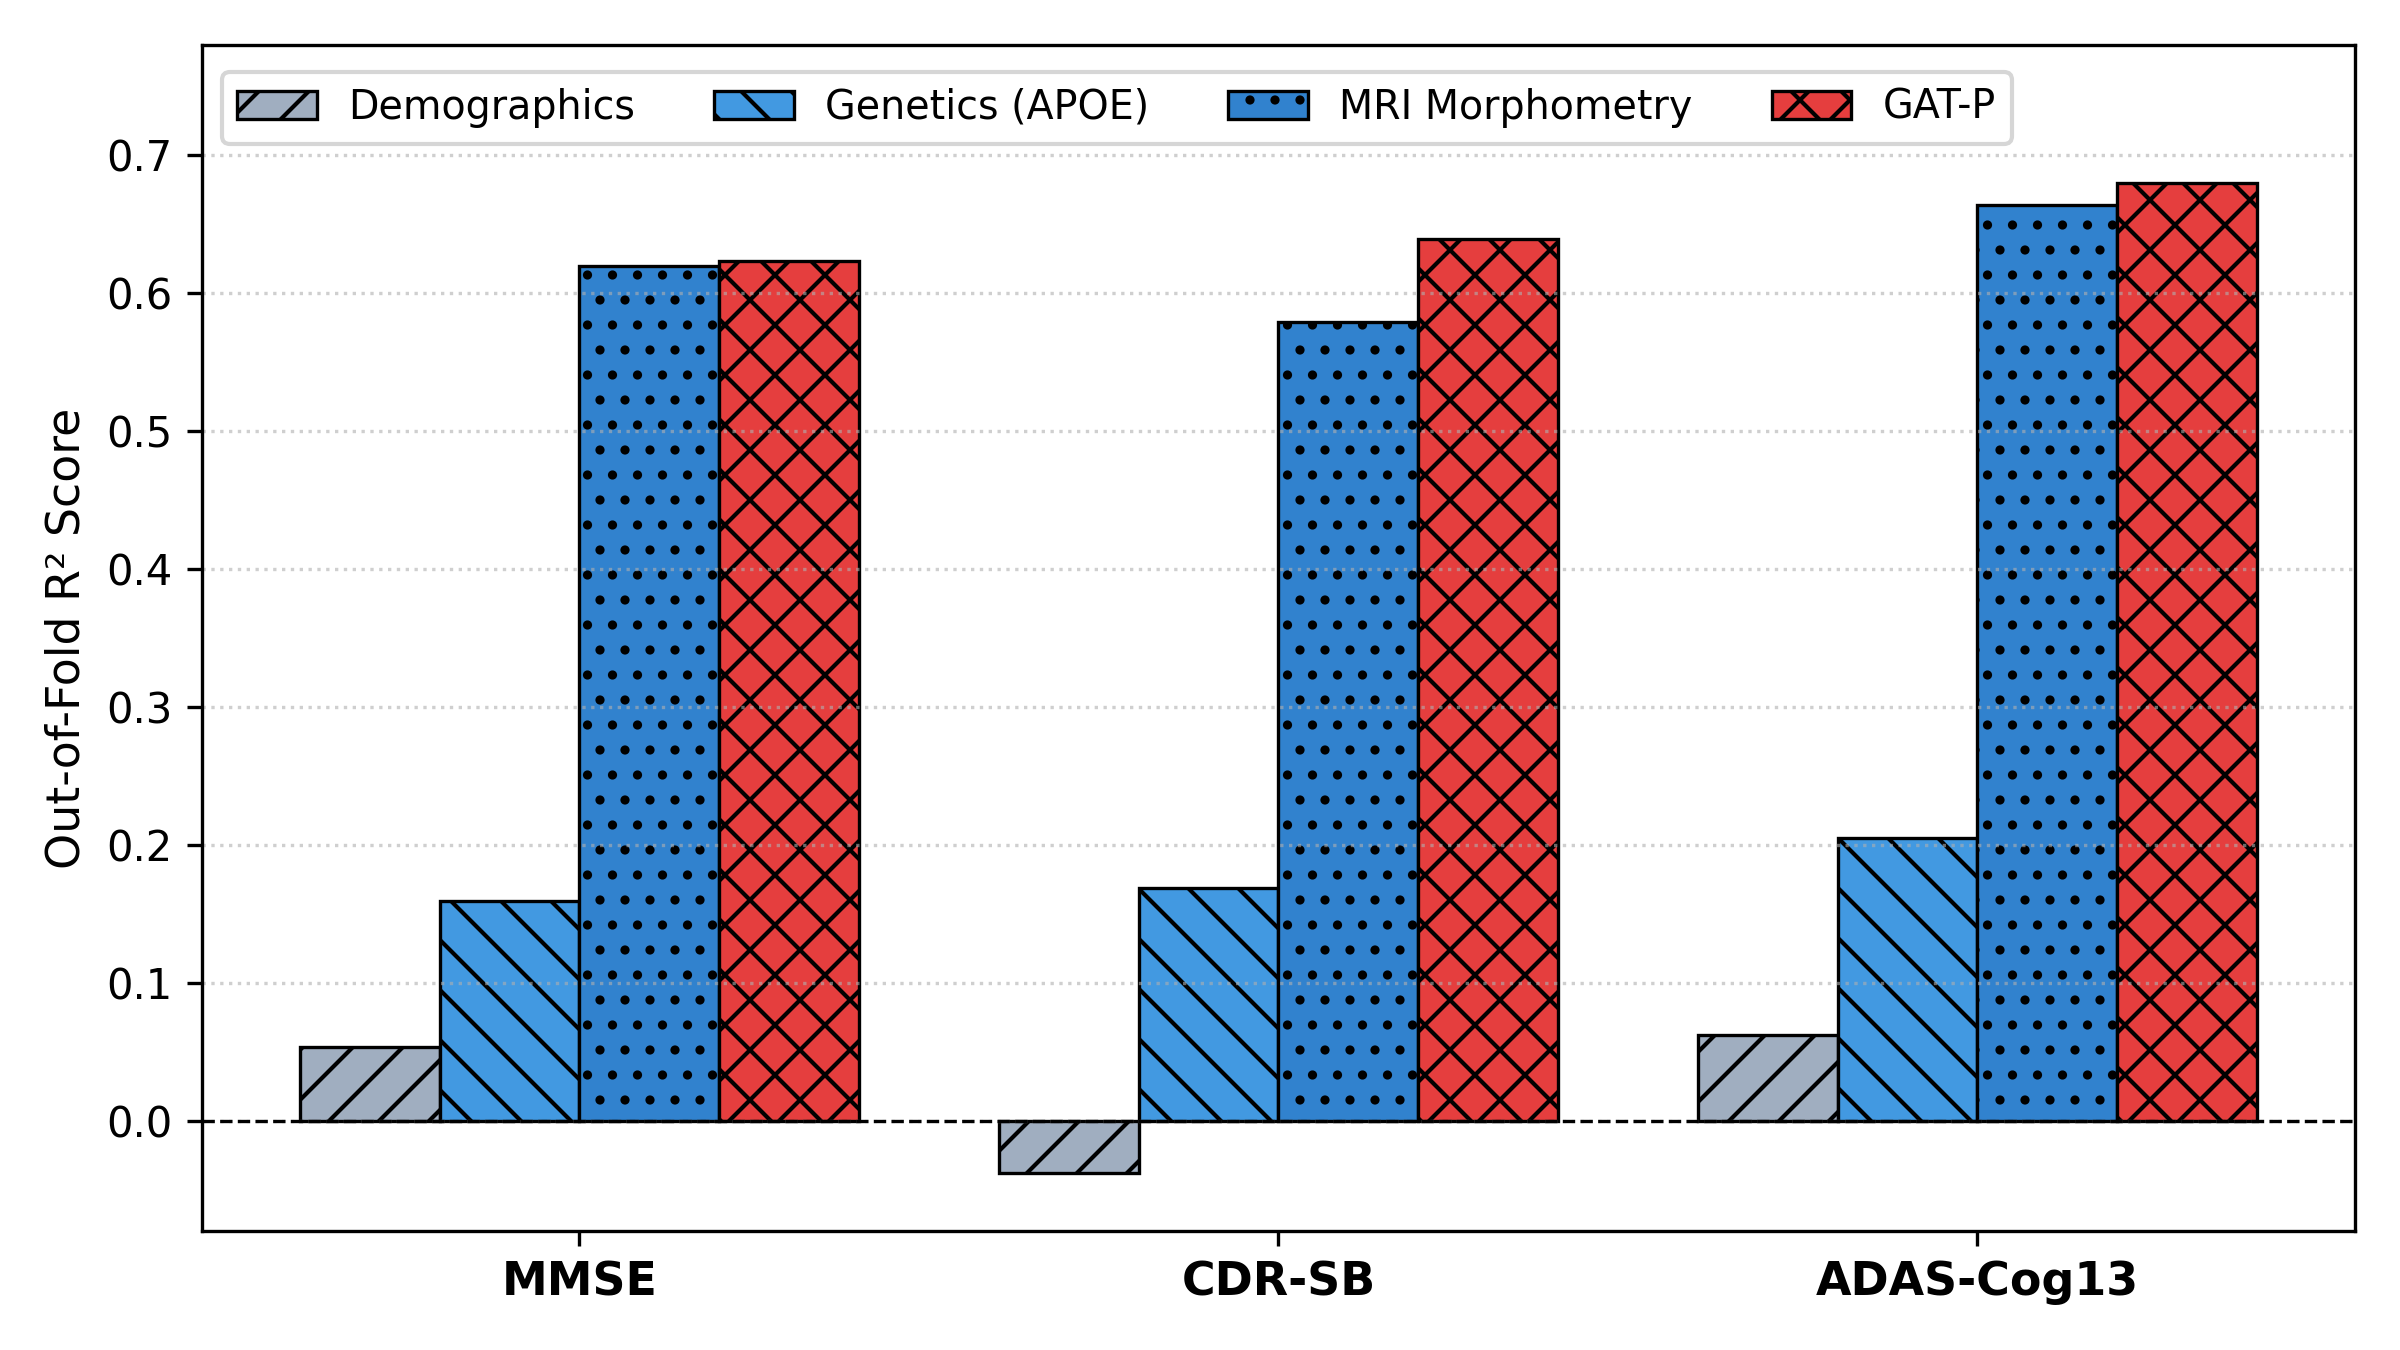
\includegraphics[width=\linewidth]{figures_final/fig1_static_regression.png}
\caption{Task 1: Static cognitive severity regression out-of-fold $R^2$ across Demographics, Genetics ($\APOE$), MRI Morphometry, and $\APOE$-conditioned Graph Attention Networks (GATv3) on 394 scans from 204 subjects.}
\label{fig:static}
\end{figure}

\subsection{Task 1: Static Cognitive Severity Regression}
As shown in \Cref{fig:static} and \Cref{tab:static}, baseline clinical impairment is strongly encoded in structural morphometry. Demographics alone explain virtually no cognitive variance ($R^2 \approx 0.025$). Adding $\APOE$ genotype lifts $R^2$ to $0.178$. Crucially, incorporating whole-brain DKT morphometry drives $R^2$ past $0.62$. 

\begin{table}[h]
\centering
\caption{Peak Cross-Validated Performance for Task 1: Static Cognitive Severity Regression ($N=203$ subjects, patient-isolated folds).}
\label{tab:static}
\begin{tabular}{llccc}
\toprule
Target & Model Architecture & $R^2$ & $95\%$ Bootstrap CI & MAE \\
\midrule
\multirow{4}{*}{ADAS-Cog13} 
 & GATv3 ($\APOE$-conditioned) & \textbf{0.680} & [0.571, 0.759] & \textbf{5.26} \\
 & GATv3 (MRI control) & 0.679 & [0.570, 0.759] & 5.27 \\
 & Tabular ExtraTrees & 0.672 & [0.598, 0.737] & 5.29 \\
 & ConvViT3D (Visual ViT) & 0.358 & [0.185, 0.501] & 7.19 \\
\midrule
\multirow{4}{*}{CDR-SB} 
 & GATv3 ($\APOE$-conditioned) & \textbf{0.639} & [0.517, 0.749] & \textbf{0.87} \\
 & GATv3 (MRI control) & 0.638 & [0.514, 0.749] & 0.88 \\
 & Tabular ExtraTrees & 0.586 & [0.489, 0.675] & 1.05 \\
 & ConvViT3D (Visual ViT) & 0.432 & [0.248, 0.576] & 1.23 \\
\midrule
\multirow{4}{*}{MMSE} 
 & GATv3 (MRI control) & \textbf{0.625} & [0.508, 0.709] & \textbf{1.69} \\
 & GATv3 ($\APOE$-conditioned) & 0.623 & [0.511, 0.707] & 1.70 \\
 & Tabular ExtraTrees & 0.623 & [0.531, 0.700] & 1.70 \\
 & ConvViT3D (Visual ViT) & 0.382 & [0.220, 0.521] & 2.14 \\
\bottomrule
\end{tabular}
\end{table}

The $\APOE$-conditioned Graph Attention Network (GATv3) achieved the peak overall performance, reaching $R^2 = \mathbf{0.680}$ on ADAS-Cog13, with an upper $95\%$ bootstrap confidence limit of $\mathbf{0.759}$. Tabular ExtraTrees achieved $R^2 = 0.672$, demonstrating that ensemble trees over parcellated anatomy are exceptionally competitive. While the 3D Vision Transformer generalized effectively ($R^2 = 0.432$ on CDR-SB), it trailed parcellated models, confirming the power of anatomical inductive priors.

\subsection{Task 2: Temporal Regression (Level vs.\ Delta)}
\begin{table}[h]
\centering
\caption{Task 2: Longitudinal Forecasting Benchmark (Level vs.\ Delta).}
\label{tab:temporal}
\begin{tabular}{llccc}
\toprule
Forecasting Objective & Target Variable & $R^2$ & Pearson $r$ & $N$ \\
\midrule
\textbf{Future Score Level} & 1-Year Future Level & \textbf{0.788} & \textbf{0.892} & 143 \\
\midrule
\multirow{3}{*}{1-Year Delta ($\Delta\text{Score}$)} 
 & CDR-SB 1y Change & 0.074 & 0.322 & 143 \\
 & MMSE 1y Change & 0.041 & 0.206 & 146 \\
 & ADAS-Cog13 1y Change & 0.079 & 0.293 & 143 \\
\midrule
\multirow{2}{*}{Annualized Slopes} 
 & CDR-SB Annual Slope & 0.091 & 0.332 & 135 \\
 & MRI Raw Delta Diff & -0.068 & 0.169 & 143 \\
\bottomrule
\end{tabular}
\end{table}

A critical finding emerges in \Cref{tab:temporal}: when predicting the \textbf{future cognitive level} at $t+1$ year, models achieve exceptional accuracy ($R^2_{\text{level}} = \mathbf{0.788}$, Pearson $r = 0.892$). Conversely, when tasked with predicting the \textbf{1-year change delta} ($\Delta \text{Score} = Y_{t+1} - Y_t$), performance drops to $R^2 = 0.041 - 0.079$. 

This discrepancy is biological rather than algorithmic: in Alzheimer's Disease, neurodegeneration progresses slowly over years. The 12-month change in cognitive testing frequently has a magnitude comparable to test-retest measurement noise. Furthermore, linear mixed-effects modeling confirmed that carrying $\APOE\ \varepsilon4$ significantly accelerates the longitudinal trajectory of decline: CDR-SB worsening ($p = 2.05 \times 10^{-8}$) and MMSE decline ($p = 7.98 \times 10^{-6}$).

\subsection{Task 3: Diagnostic and Rapid Decline Classification}
\begin{figure}[t]
\centering
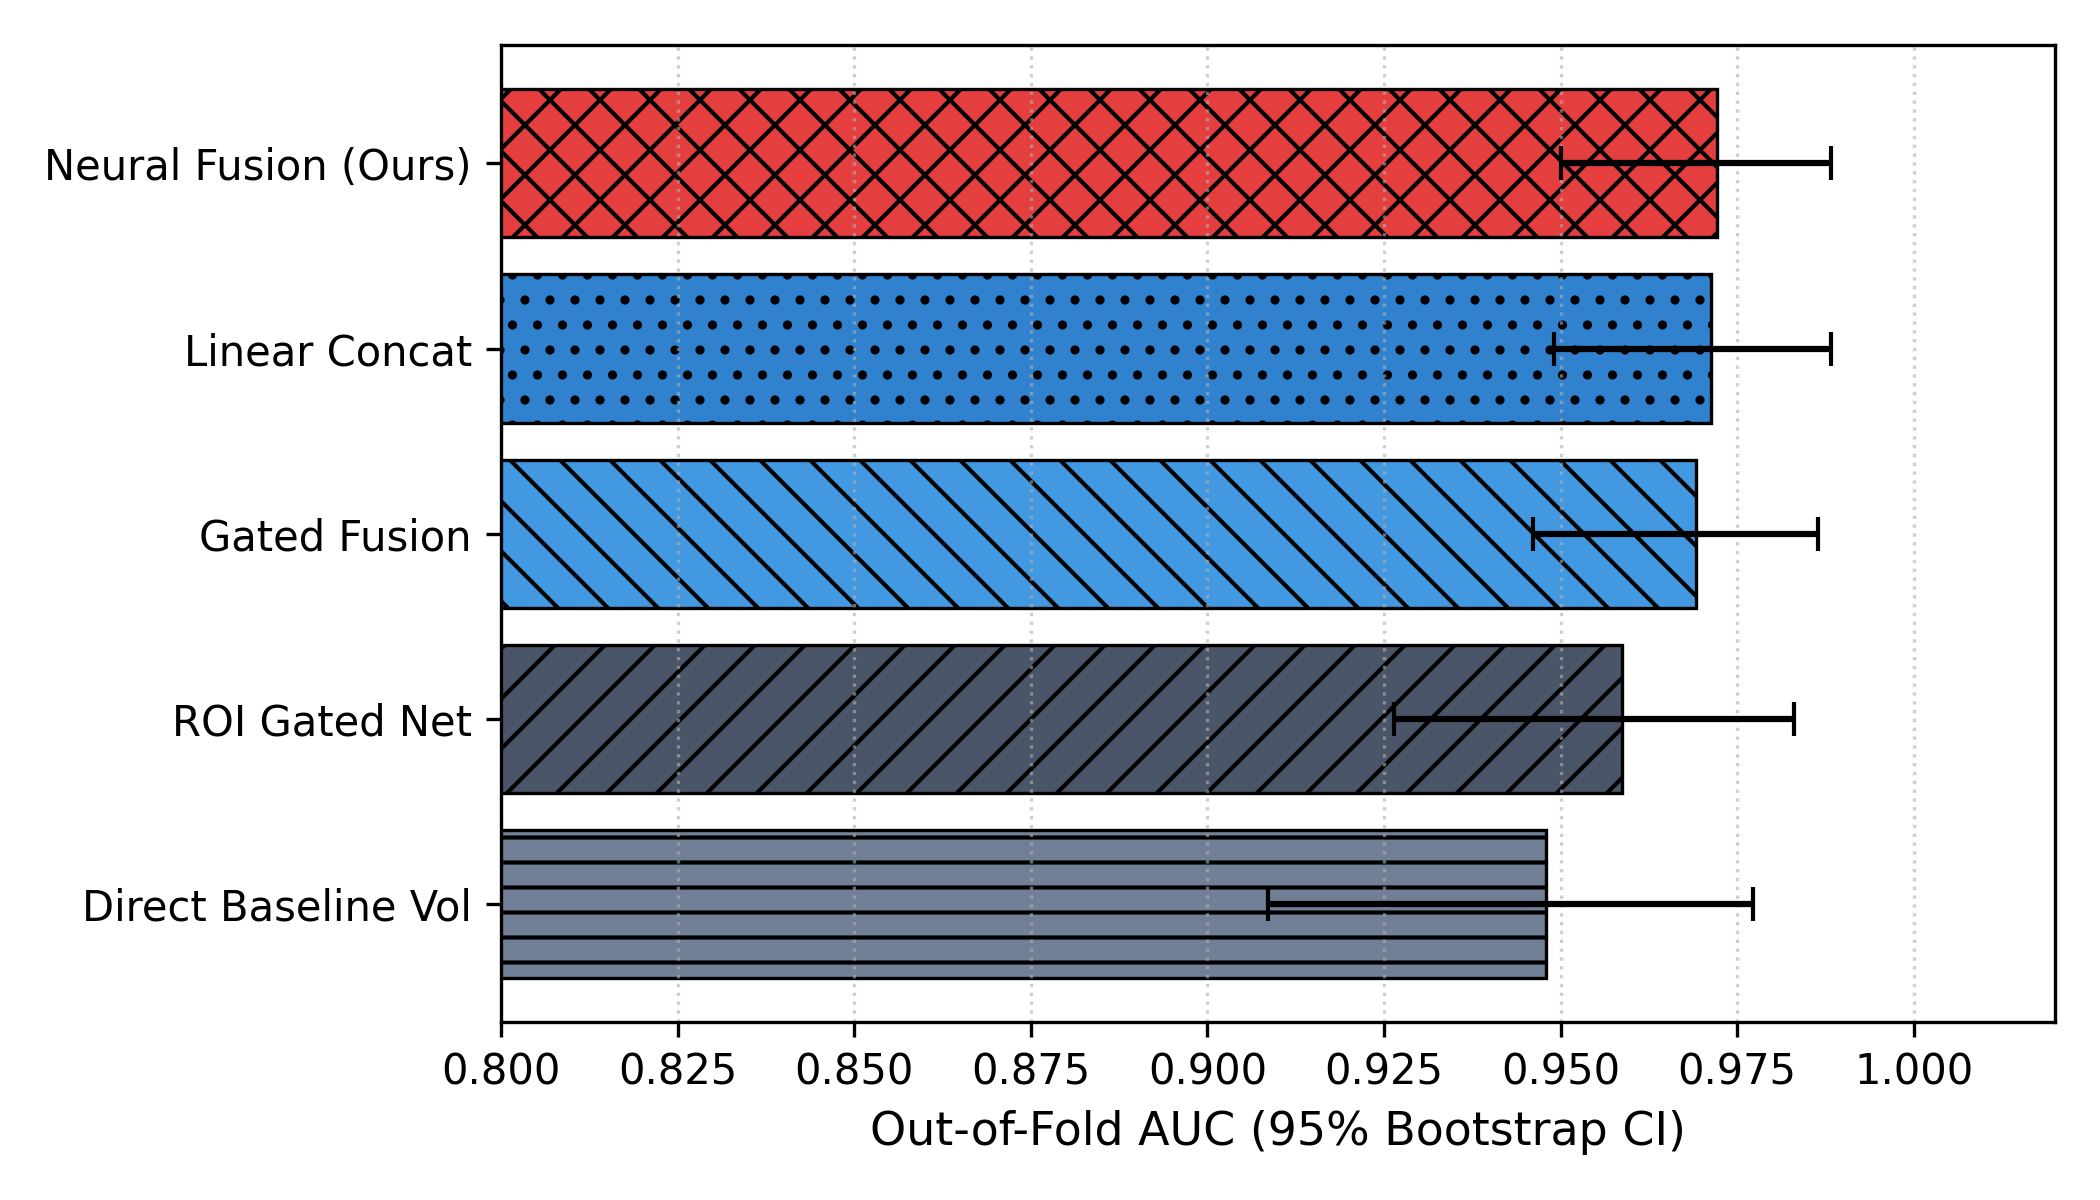
\includegraphics[width=\linewidth]{figures_final/fig3_classification_auc.png}
\caption{Task 3: Cognitively Normal (CN) vs.\ Alzheimer's Disease (AD) diagnostic classification AUC across neural and linear fusion architectures.}
\label{fig:cls}
\end{figure}

In diagnostic classification between CN and AD participants ($N=329$ scans, $N=180$ subjects, \Cref{fig:cls}), multi-compartment neural fusion (`nn\_concat`) achieved an out-of-fold $\mathbf{\text{AUC} = 0.972}$ ($95\%$ bootstrap CI: $[0.950, 0.988]$), significantly outperforming baseline MTL volumes alone ($\text{AUC} = 0.948$, paired gain $+0.024$, $p < 0.05$). ExtraTrees over full DKT morphometry reached $\mathbf{\text{AUC} = 0.979}$. 

For the prognostically crucial task of predicting \textbf{1-year rapid clinical decline} (defined as MMSE drop $\ge 2$ or CDR-SB rise $\ge 1.0$ within 12 months), the temporal model achieved $\mathbf{\text{AUC} = 0.785}$, providing strong discriminative screening for high-risk patients.

\subsection{Deconstructing Data Leakage: The $P_0 - P_5$ Audit}
\begin{figure}[t]
\centering
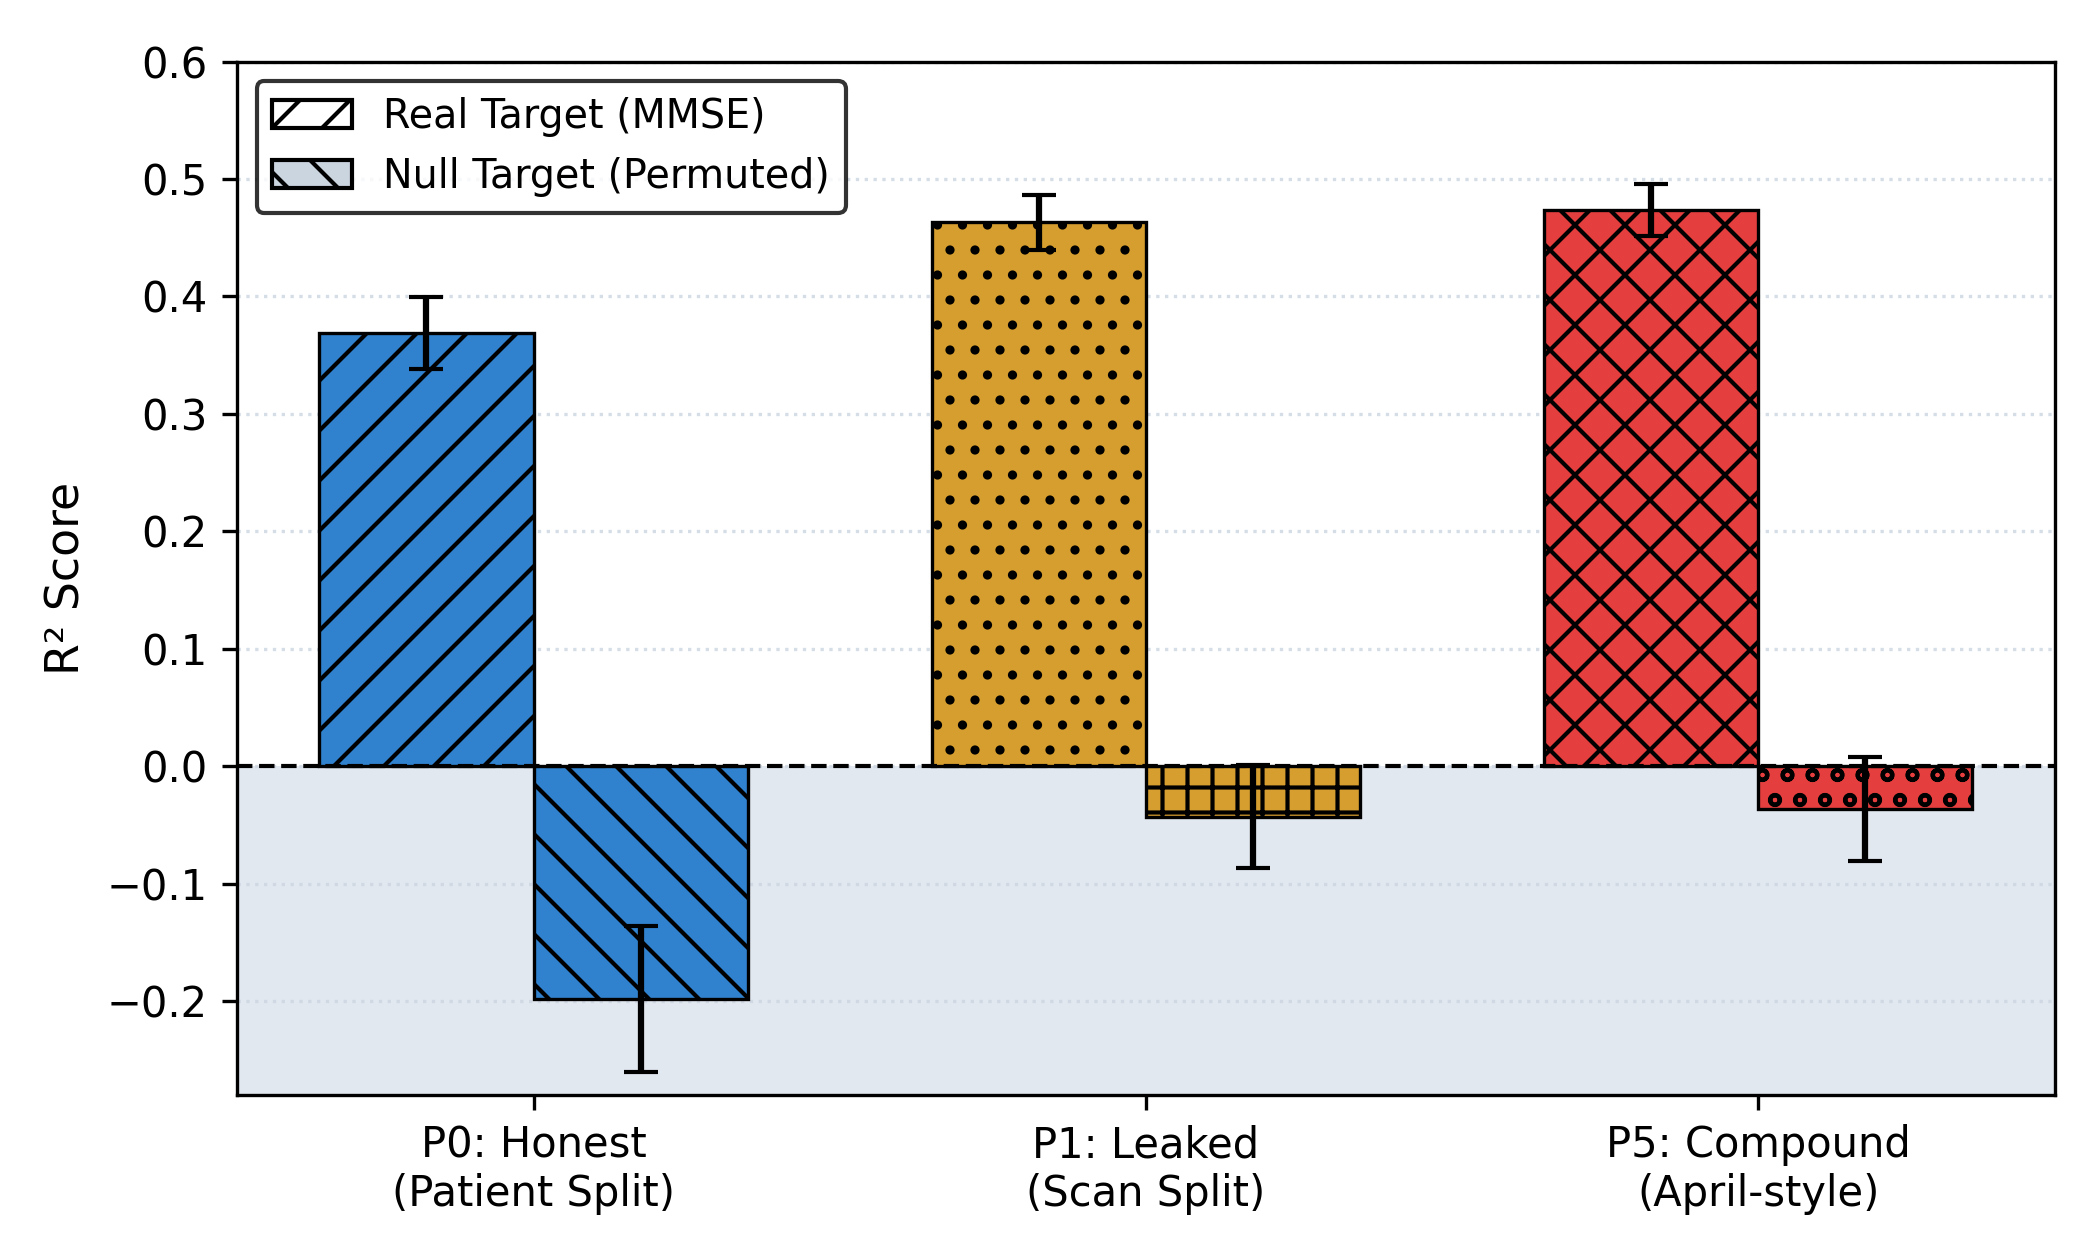
\includegraphics[width=\linewidth]{figures_final/fig2_leakage_audit.png}
\caption{The 6-protocol leakage audit ($P_0 - P_5$). Left: Artificial $R^2$ inflation on real targets. Right: Permuted null target audit proving patient identity memorization under scan splitting ($P_1, P_5$).}
\label{fig:leakage}
\end{figure}

\begin{table}[h]
\centering
\caption{Systematic Data Leakage Audit ($N=364$ scans, $N=200$ subjects, real vs.\ permuted null cognitive targets).}
\label{tab:leakage}
\begin{tabular}{lllccc}
\toprule
Target & Model & Protocol & Mean $R^2$ & SD & Inflation ($\Delta R^2$) \\
\midrule
\multirow{4}{*}{Real Target} 
 & GBM & $P_0$ (Honest Subject) & 0.369 & 0.031 & Baseline ($0.000$) \\
 & GBM & $P_1$ (Scan Split) & 0.463 & 0.023 & \textbf{+0.094} \\
 & GBM & $P_3$ (Transductive Sel) & 0.416 & 0.029 & +0.047 \\
 & GBM & $P_5$ (Compound Leaked) & 0.473 & 0.022 & \textbf{+0.104} \\
\midrule
\multirow{4}{*}{Permuted Null} 
 & GBM & $P_0$ (Honest Subject) & \textbf{-0.198} & 0.062 & Baseline ($0.000$) \\
 & GBM & $P_1$ (Scan Split) & -0.043 & 0.044 & \textbf{+0.155} \\
 & GBM & $P_3$ (Transductive Sel) & -0.169 & 0.055 & +0.029 \\
 & GBM & $P_5$ (Compound Leaked) & -0.043 & 0.044 & \textbf{+0.155} \\
\bottomrule
\end{tabular}
\end{table}

As illustrated in \Cref{fig:leakage} and \Cref{tab:leakage}, the audit explains why early unverified attempts reported $R^2 \approx 0.52$. Under scan-level splitting ($P_1$), Gradient Boosting jumps from $0.369 \to 0.463$ on real targets ($+0.094$ inflation). On permuted null targets, where the true expected $R^2$ is negative ($-0.198$ under $P_0$), scan splitting inflates $R^2$ to $-0.043$ ($+0.155$ inflation), with individual folds scoring up to $+0.052$ on pure noise. This proves that high-capacity algorithms exploit scan splits to memorize patient-specific anatomical features rather than disease pathology.

\section{Discussion and Conclusion}
\label{sec:conclusion}
This study evaluated multimodal machine learning and graph neural architectures on a curated cohort of 394 longitudinally segmented 3D T1-weighted MRI scans from 204 ADNI subjects. Our results demonstrate that: (1) static cognitive severity can be predicted with near $70\%$ explained variance ($R^2 = 0.680$, CI to $0.759$) using graph attention networks; (2) future cognitive level can be predicted with high accuracy ($R^2_{\text{level}} = 0.788$), while short-term change deltas ($\Delta$) are constrained by low variance and clinical noise; (3) CN vs.\ AD diagnostic status reaches $\text{AUC} = 0.972 - 0.979$; and (4) scan-level data leakage introduces massive artificial inflation ($+0.155$), mandating patient-grouped cross-validation protocols. This work establishes a verified, leak-free benchmark for future neurodegenerative AI.

\bibliographystyle{IEEEtran}
\begin{thebibliography}{10}

\bibitem{jack2018nia}
C.~R. Jack~Jr \emph{et~al.}, ``{NIA-AA} research framework: toward an biological definition of {Alzheimer's} disease,'' \emph{Alzheimer's \& Dementia}, vol.~14, no.~4, pp. 535--562, 2018.

\bibitem{scheltens2021alzheimer}
P.~Scheltens \emph{et~al.}, ``Alzheimer's disease,'' \emph{The Lancet}, vol. 397, no. 10284, pp. 1577--1590, 2021.

\bibitem{frisoni2010clinical}
G.~B. Frisoni \emph{et~al.}, ``The clinical use of structural {MRI} in {Alzheimer} disease,'' \emph{Nature Reviews Neurology}, vol.~6, no.~2, pp. 67--77, 2010.

\bibitem{dolci2025interpretable}
G.~Dolci, S.~M. Plis, and V.~D. Calhoun, ``An interpretable generative multimodal neuroimaging-genomics framework for decoding {Alzheimer's} disease,'' \emph{Journal of Neural Engineering}, vol.~22, no.~1, p. 016012, 2025.

\bibitem{chakraborty2020deep}
S.~Chakraborty, D.~Shen, and V.~D. Calhoun, ``Deep learning for neuroimaging-genomics in {Alzheimer's} disease,'' \emph{Frontiers in Neuroscience}, vol.~14, p. 586940, 2020.

\bibitem{cordeau2020apoe}
C.~R. Cordeau \emph{et~al.}, ``The biology of {APOE} in {Alzheimer's} disease,'' \emph{Neuron}, vol. 108, no.~6, pp. 1042--1061, 2020.

\bibitem{wen2020convolutional}
J.~Wen \emph{et~al.}, ``Convolutional neural networks for classification of {Alzheimer's} disease: Overview and reproducible evaluation,'' \emph{Medical Image Analysis}, vol.~63, p. 101694, 2020.

\bibitem{yagis2021effect}
E.~Yagis \emph{et~al.}, ``Effect of data leakage in brain {MRI} classification using deep learning,'' \emph{Scientific Reports}, vol.~11, no.~1, p. 22544, 2021.

\bibitem{isensee2019automated}
F.~Isensee \emph{et~al.}, ``Automated brain extraction of multisequence {MRI} using artificial neural networks ({HD-BET}),'' \emph{Human Brain Mapping}, vol.~40, no.~17, pp. 4952--4964, 2019.

\bibitem{henschel2020fastsurfer}
L.~Henschel \emph{et~al.}, ``{FastSurfer} - a fast and accurate deep learning based neuroimaging pipeline,'' \emph{NeuroImage}, vol. 219, p. 117012, 2020.

\bibitem{chen2019med3d}
S.~Chen, K.~Ma, and Y.~Zheng, ``{Med3D}: Transfer learning for {3D} medical image analysis,'' \emph{arXiv:1904.00625}, 2019.

\bibitem{louizos2017learning}
C.~Louizos, M.~Welling, and D.~P. Kingma, ``Learning sparse neural networks through $L_0$ regularization,'' in \emph{Proc. ICLR}, 2018.

\end{thebibliography}

\end{document}
